\documentclass[a4paper,11pt,twocolumn]{article}
\usepackage[utf8]{inputenc}
%\usepackage[italian]{babel}

%\usepackage{lipsum}
\usepackage{float}
\usepackage{graphicx}
\usepackage[font=small,labelfont=bf]{caption}
\usepackage{multirow}
\usepackage{hyphenat}
\usepackage{sectsty}
%\usepackage{subfigure}
%\usepackage{color}
%\usepackage[dvipsnames]{xcolor}
%\sectionfont{\bfseries\Large\raggedright}
\usepackage{hyperref}
\allsectionsfont{\raggedright}
\graphicspath{ {images/} }

\usepackage[backend=bibtex,sorting=none]{biblatex}
\addbibresource{bibliography.bib}

%\usepackage[T1]{fontenc}

\pagestyle{headings}


\title{Detection of a transiting Hot Jupiter around WASP-44}
\author{Adriana Barbieri \and Alessandro Bianchetti}

\begin{document}
\maketitle

\begin{abstract}

\emph{In the following report we work on WASP-44 b, an exoplanet orbiting 
arounf its G-type mother star, located in the constellation of Cetus. 
We first take a look at its atmospheric parameters and derive mass and 
radius. Then, we correct for limb darkening effect. We also take some 
images taken by Copernico at the Asiago Observatory into consideration and, 
after proper correction, we use them to extract the light curve of the 
alleged planet.}

\end{abstract}

\section{Introduction}

Confirmed exoplanets are growing in number year by year, and transit method 
is nowadays a widely spread method. Most planets nowadays are discovered 
by tracing the lightcurve and searching for any sign of a weakening in the 
flux.
\begin{figure}[H]
    \centering  
    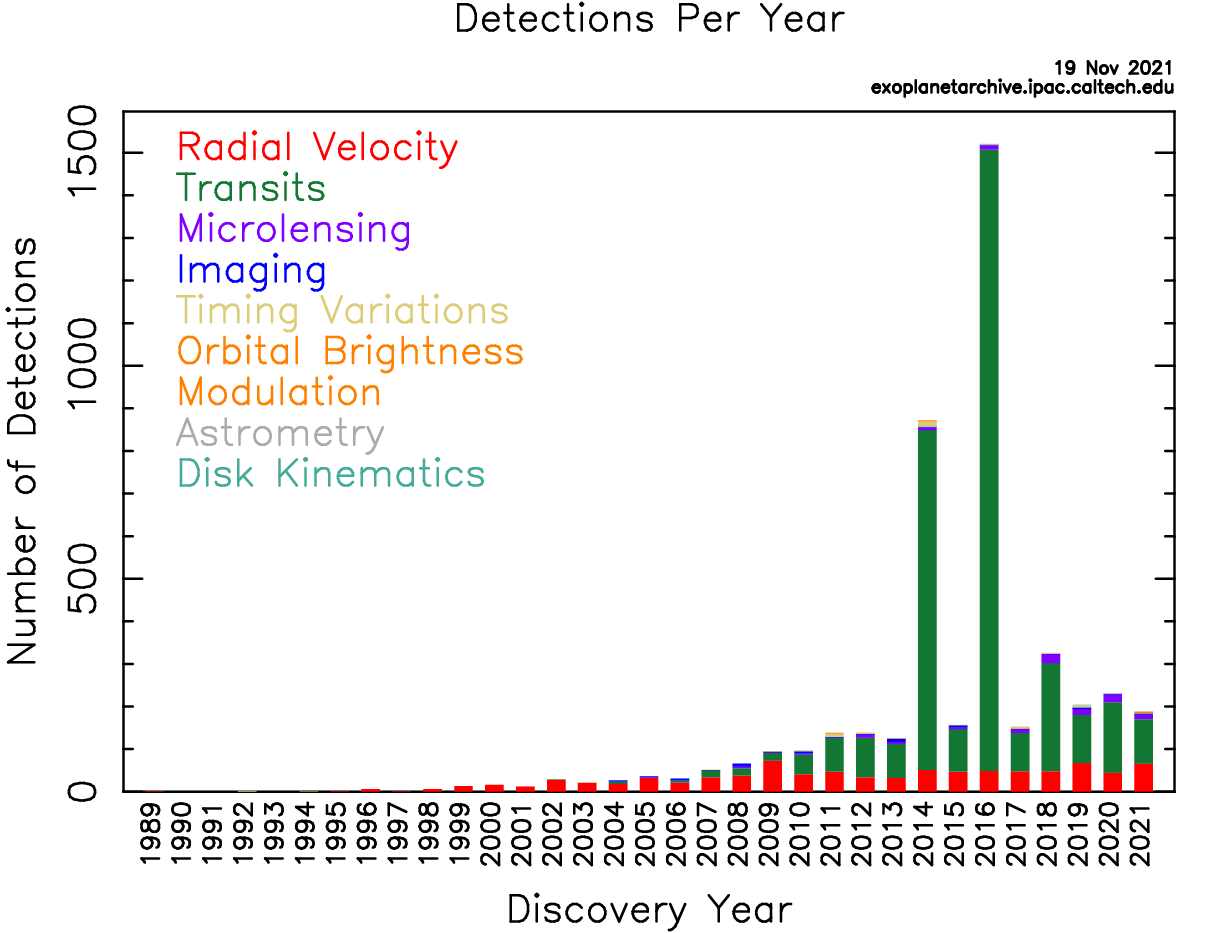
\includegraphics[scale=0.15, angle=0]{../pictures/exo_dischist.png}
    \caption*{\textit{ https://exoplanetarchive.ipac.caltech.edu/}}
\end{figure}
In this report we focus on WASP-44 b, a Jupyter-size planet orbiting around 
a G-type star, located in the constellation of Cetus.
Among the numerous available reports on the planet, we decided to make a 
conservative choice and avoid any result which is not inferred via 
spectroscopy. This leads us to rule out several papers about the object, and 
only work with the discovery paper \cite*{Anderson}. In this paper, estimates 
of the atmospheric parameters of WASP-44 are provided via an analysis of 
the width of spectral lines.

\section{Instruments}

Bla bla



\section{Theoretical recap}

[- a brief overview of the transit method
- a comment on the bias of the transit method (big planets, close to the star)]




\subsection{Bla bla}

\section{Data analysis}

\subsection{Inferring mass and radius}

The $H_{\alpha}$ line was used to determine the effective temperature (Teff ),
while the $NaI$ D and $MgI$ b lines were used as surface gravity
($\log{g^*}$) diagnostics. The elemental abundances, including $[Fe/H]$ 
were determined from equivalent width measurements of several clean and 
unblended lines. This led to proper estimation of the atmospheric parameter 
triplet $T_{eff}$, $\log{g^*}$ and $[Fe/H]$. \cite*{Anderson} mentions that the quoted errors 
include statistical uncertainties and does not say anything specific about 
systematic contributions. In the same conservative spirit we previously 
showed, we add in quadrature a further term to the errors of all three 
parameters according to \cite*{Sousa}. We're in fact more interested in an accurate result 
rather than a precise one.
This leads to the following results 
\begin{center}
    \begin{tabular}{|c|c|c|}
    \hline
    $T_{eff}$ (K) & $\log{g^*}$ & $[Fe/H]$ \\
    $5400 \pm 162$ & $4.5 \pm 0.2$ & $0.06 \pm 0.11$ \\
    \hline
    \end{tabular}
    \end{center}


\subsection{Limb darkening correction}

\subsection{Bias and flat field correction}

\subsection{Extracting the light curve}


\section{Conclusions}

Bla bla




\printbibliography

\end{document}